\documentclass[12pt, a4paper, fleqn]{article}

\usepackage{fontspec}
\usepackage{amsmath}
\usepackage{mathtext}
\usepackage{indentfirst}
\usepackage{enumitem}
\usepackage{minted}
\usepackage{ragged2e}
\usepackage{xcolor}
\usepackage{graphicx}
\usepackage{polyglossia}
\usepackage[a4paper, top = 2.5 cm, bottom = 2.5 cm, left = 2.5 cm, right = 2.5 cm]{geometry}

\setmainlanguage{russian}
\setotherlanguage{english}
\newfontfamily\russianfont[Script = Cyrillic]{Arial}
\let\russianfonttt\ttfamily

\begin{document}

\begin{titlepage}
	\centering
	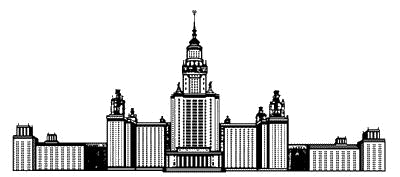
\includegraphics[scale = 0.7]{msutitlepic.png} \par
	\vspace{0.5 cm}
	{\large МОСКОВСКИЙ ГОСУДАРСТВЕННЫЙ УНИВЕРСИТЕТ имени~М.В.~ЛОМОНОСОВА \par}
	{\large ФАКУЛЬТЕТ ВЫЧИСЛИТЕЛЬНОЙ МАТЕМАТИКИ И КИБЕРНЕТИКИ \par}
	\rule[0.5ex]\linewidth{1pt} \par
	{\normalsize КАФЕДРА АВТОМАТИЗАЦИИ СИСТЕМ ВЫЧИСЛИТЕЛЬНЫХ КОМПЛЕКСОВ \par}

	\vspace{4 cm}
	{\large\textbf{Отчёт о выполнении задания №2\\по курсу "Имитационное моделирование в исследовании и разработке информационных систем"} \par}
	\vspace{0.5 cm}
	{\Large Построение и исследование имитационной модели \par}
	
	\vfill
	{\raggedleft\Large Мирошник В.А. \par}
	{\raggedleft\Large 321 группа \par}
	
	\vspace{2 cm}
	{\large Москва, 2017}
\end{titlepage}

\newpage
\raggedright
\large

\section{Постановка задачи}
\justifying

\noindent \textbf{Общие положения:} \par
\vspace{0.3cm} \noindent Дано описание исследуемой системы на естественном языке, заданы цели исследования системы. \par
\vspace{0.3cm}
\noindent \textbf{Требуется:}

\begin{itemize}[leftmargin=0.5cm]
	\item построить концептуальную модель (указать, какие упрощающие предположения принимаются, описать структуру системы, взаимодействие между компонентами);
	\item построить имитационную модель в системе моделирования по выбору; 
	\item провести эксперименты с моделью в соответствии с целью исследования;
	\item сделать выводы и составить отчет о работе.
\end{itemize}

\section{Концептуальная модель}

В кафе университета особенно большой наплыв клиентов наблюдается с 11:30 до 13:00, когда они прибывают группами по 1, 2, 3, 4 человека с вероятностями 0.5, 0.3, 0.1, 0.1 соответственно. Интервалы между прибытиями групп распределены экспоненциально со средним значением 30 сек. Изначально клиенты в системе отсутствуют. Каждый клиент в отдельности выбирает один из трех машрутов:

\begin{itemize}
	\item пункт выдачи горячих блюд, пункт выдачи напитков, касса с вероятностью 0.8;
	\item пункт выдачи холодных закусок, пункт выдачи напитков, касса с вероятностью 0.15;
	\item пункт выдачи напитков, касса с вероятностью 0.05.
\end{itemize}

На выдаче горячих блюд и холодных закусок клиентов обслуживает какое-то количество сотрудников. В пункте выдачи напитков считаем, что очереди нет. \par
В системе присутствует несколько касс, к каждой из которых выстраивается очередь. Переход клиентов из одной очереди в другую невозможен. Клиенты, желающие рассчитаться, присоединяются к самой короткой очереди. Все очереди в системе имеют дисциплину обслуживания FIFO. Для упрощения построения имитационной модели считаем, что очередь общая ко всем кассам, а первый клиент в очереди начинает рассчитываться после того, как освободилась любая касса. \par
На каждом пункте выдачи клиент обслуживается определенное количество времени (ВО), которое является случайной величиной, распределенной равномерно, и накапливает время оплаты (НВО) на кассе, которое тоже является равномерно распределенной случайной величиной. На пункте выдачи горячих блюд ВО\textasciitilde U(50, 120), НВО\textasciitilde U(20, 40), на выдаче холодных закусок ВО\textasciitilde U(60, 180), НВО\textasciitilde U(5, 15), на выдаче напитков ВО\textasciitilde U(5, 20), НВО\textasciitilde U(5, 10). Во всех случаях считается, что случайные величины независимы друг от друга. \par
Прогон модели должен соответствовать 90 мин работы системы. Клиенты, не обслуженные по истечению 90 мин работы системы, не рассматриваются.

\section{Цели исследования}

Требуется определить следующие оценки работы системы:

\begin{itemize}
	\item среднюю и максимальную задержку в очереди к пунктам выдачи горячих блюд, холодных закусок и кассам;
	\item среднее по времени и максимальное число клиентов в очереди к пунктам выдачи горячих блюд и холодных закусок, а также среднее по времени и максимальное общее число клиентов в очереди к кассам;
	\item среднюю и максимальную общую задержку во всех очередях для каждого из трех типов клиентов;
	\item суммарную среднюю общую задержку для всех клиентов, которая определяется весовыми коэффициентами отдельных средних общих задержек по соответствующим вероятностям их возникновения;
	\item среднее по времени и максимальное общее число клиентов во всей системе. 
\end{itemize}

Также нужно выполнить прогоны семи вариантов модели и дать рекомендации относительно наилучшего распределения сотрудников для каждой из них. 

\section{Экспериментальное исследование модели}

Имитационная модель была построена в системе моделирования SimPy. С кодом программы можно ознакомиться по ссылке.

\begin{enumerate}
	\item Базовая ситуация: 1 сотрудник на выдаче горячих блюд, 1 сотрудник на выдаче холодных закусок, 2 кассы. \\
	
	\noindent На выдаче горячих блюд: \\
	Максимальное время задержки 68 мин 6 сек, среднее время задержки 32 мин 26 сек \\
	Максимальное количество клиентов 247, среднее время в очереди 33 мин 48 сек\\
	На выдаче холодных блюд: \\ 
	Максимальное время задержки 15 мин 35 сек, среднее время задержки 6 мин 5 сек \\
	Максимальное количество клиентов 9, среднее время в очереди 7 мин 58 сек \\
	На кассах: \\
	Максимальное время задержки 0 мин 14 сек, среднее время задержки 0 мин 0 сек \\
	Максимальное количество клиентов 3, среднее время в очереди 0 мин 29 сек

	Для посетителей первого типа: \\
	Максимальное время задержки во всех очередях 65 мин 10 сек, среднее 31 мин 19 сек \\
	Для посетителей второго типа: \\
	Максимальное время задержки во всех очередях 14 мин 24 сек, среднее 5 мин 51 сек \\
	Для посетителей третьего типа: \\
	Максимальное время задержки во всех очередях 0 мин 14 сек, среднее 0 мин 1 сек \\
	Суммарная средняя задержка 25 мин 56 сек

	Для всех посетителей: \\
	Максимальное число в системе 253 \\
	Среднее по времени нахождение в системе 20 мин 6 сек \\
\end{enumerate}

\section{Выводы}

\justifying
\hspace{0.4 cm}
Как мы видим, измененная программа на данной конфигурации компьютера работает почти в 6 раз быстрее, чем первоначальная. Причина кроется в специфике расположения данных в памяти и работы памяти разных уровней. В задании мы работали с двумерными массивами, содержащими по 100 миллионов элементов каждый. В линейной памяти массив хранится построчно: сначала идет первая строка, за ней вторая и так далее. Если мы будем обращаться к элементам массива последовательно, то будет велика вероятность того, что следующий элемент встретится в кэше процессора, так как процессоры используют технологию кэширования, загружая блоки данных из оперативной памяти. Таким образом, будет существенно уменьшено количество обращений к "медленной" оперативной памяти и увеличено \textemdash ~к "быстрой" кэш-памяти, поэтому программа будет выполняться быстрее. В этом мы и убедились после изменения порядка обхода массивов. \par
Тем не менее, это не единственный способ повысить быстродействие программы. Еще при компиляции программы можно указать один из флагов оптимизации и предоставить компилятору провести оптимизационную работу самостоятельно. К примеру, использование флага оптимизации -О3 компилятора gcc позволяет ускорить работу исходной программы примерно в 3 раза \textemdash ~до 4.4 сек, а для измененной программы время выполнения составит 1.3 сек. \par
На основе вышесказанного можно сделать следующий вывод: чтобы писать хороший эффективный код, нужно знать и принимать во внимание многие низкоуровневые особенности работы компьютера, изучать возможности используемых компиляторов и быть нацеленным на достижение максимальных результатов.

\end{document}